%NOME: Francisco Rosa Dias de Miranda
%CÓDIGO: 4402962
%CURSO: Bacharelado em Estatística
%DISCIPLINA: Laboratório de Computação e Simulação

\documentclass[a4paper,10pt]{article}
\usepackage[utf8]{inputenc}
\usepackage[portuguese]{babel}
\usepackage{amsmath}
\usepackage{amssymb}
\usepackage{graphicx}

\title{Cálculo de integrais usando o algoritmo de Metropolis-Hastings}
\author{Francisco Rosa Dias de Miranda}

\begin{document}

\maketitle

\section{Definição do Problema}

Considere a função $$g(t) = \frac{1}{c} e^{((-0.2506)(1+t))} (0.5) (1 + cos((0.6440t))$$ com $c$ sendo uma constante de normalização. O objetivo deste EP é descobrir o valor numérico com 3 dígitos significativos  para $$\gamma = \int_0^\infty f(t) g(t)dx$$ com $f(t)$ sendo uma função qualquer entrada pelo usuário.
\\
 Para calcular $\gamma$ através de um Método MCMC, geramos variáveis aleatórias para a distribuição dada pela função de densidade $g(t)$ utilizando o algoritmo de Metropolis-Hastings e  o gerador de números aleatórios nativo do R para distribuições uniforme e normal com média $\mu = 0$ e desvio padrão $\sigma = 1$.

\section{Metodologia}

Este EP foi desenvolvido em R. Como parâmetros, temos, $\sigma$, $n_0$ e n, respectivamente desvio padrão do Núcleo, número de pontos para as iterações iniciais (burn-in) e número de pontos utilizado no cálculo a integral, sendo a saída impressa na tela com os valor da integral.
\\
O algoritmo de Metropolis-Hastings é um dos exemplos mais populares de um método de Monte Carlo via Cadeias de Markov (MCMC). Abaixo encontra-se um esquema do algoritmo utilizado:

\begin{enumerate}
\item Começo com um valor inicial $x \in [0,1]$;
\item Gero um número aleatório $u$ com a distribuição proposta $h$ entre $[0,1]$;
\item Calculo a razão de Metrópolis dada por $R=\dfrac{g(u)h(x)}{g(x)h(u)}$ e determino a probabilidade de aceitação $\alpha =min\{1,R\}$;
\item Gero um número aleatório $p$ com distribuição uniforme entre $0$ e $1$ e comparo com $\alpha$;
\item Se $p \leq \alpha$, aceito $u$ como tendo distribuição $g$, atualizo o valor de $x$ fazendo $x=u$;
\item Retorno ao passo 2.
\end{enumerate}
Ele oferece uma técnica de amostragem para uma distribuição genérica P(x) que é útil em casos que é possível escrever uma expressão para a probabilidade P(x), mas o método para gerar um número aleatório dessa distribuição $x \sim P(x)$ é desconhecido.


Primeiramente, assumindo que a integral fosse decescente e convergisse, foi necessário encontrar um $t$ tal que $g(t) < 0.0009$, para que os valores de $g$ a partir daquele ponto não impactassem na precisão exigida. Para tanto, $f(15) = 0.000249773$ foi suficiente.

Para a geração de números aleatórios com distribuição normal entre 0 e 15, foi utilizado o método da transformada inversa, 
utilizando para tanto a função \textbf{qnorm} do R, que retorna a inversa da função normal (calculada numericamente) num 
ponto x. Seja $g_{norm}$ a função densidade de probabilidade normal de parâmetros $\mu=0$, ajustamos $\sigma$ de forma que $g_{norm}$ possa assumir valores maiores que 15. $\sigma = 12$ foi considerado suficiente. Portanto temos:

\[g_{norm}(0,5)=0 \textrm{ e } g_{norm}(0,9) \approx 15\]

Assim, $g^{-1}_{norm}(u)$ tem distribuição normal se $u$ tiver distribuição uniforme. Mais do que isto, se tomarmos $u$ com distribuição uniforme entre $0,5 \textrm{ e } 0,9$, teremos um gerador de números aleatórios com distribuição normal com parâmetros
 $\mu=0$ e $\sigma=12$, mas que só gera valores entre $0$ e $15$. Utilizando deste procedimento, a razão de Metropolis será:
\[R=\dfrac{g(u)f_{norm}(x)}{g(x)f_{norm}(u)}\]

Suponha que conhecemos um estágio atual $x_n$ de uma Cadeia de Markov, iremos gerar um estágio $x_{n+1}$ a partir de um candidato $x^*$, gerado a partir de uma *distribuição proposta* denotada por $Q(x^*|x_n)$ Normal($x_n,15$).

Sabemos que, para garantir a estabilidade do método para a distribuição esperada, precisamos iterar algumas vezes antes de 
atingir a convergência (a convergência é garantida para $n$ iterações, quando $n \rightarrow \infty$). No caso deste EP, nosso 
código gera 1000 iterações iniciais antes de começar a utilizar a saída para obter números com a distribuição $g(t)$ (burn-in).

\section{Teste Numérico}

Os histogramas abaixo ilustram o ajuste realizado para encontrar n0 e n convenientes para o cálculo de $\gamma$.
\begin{figure}
\centering
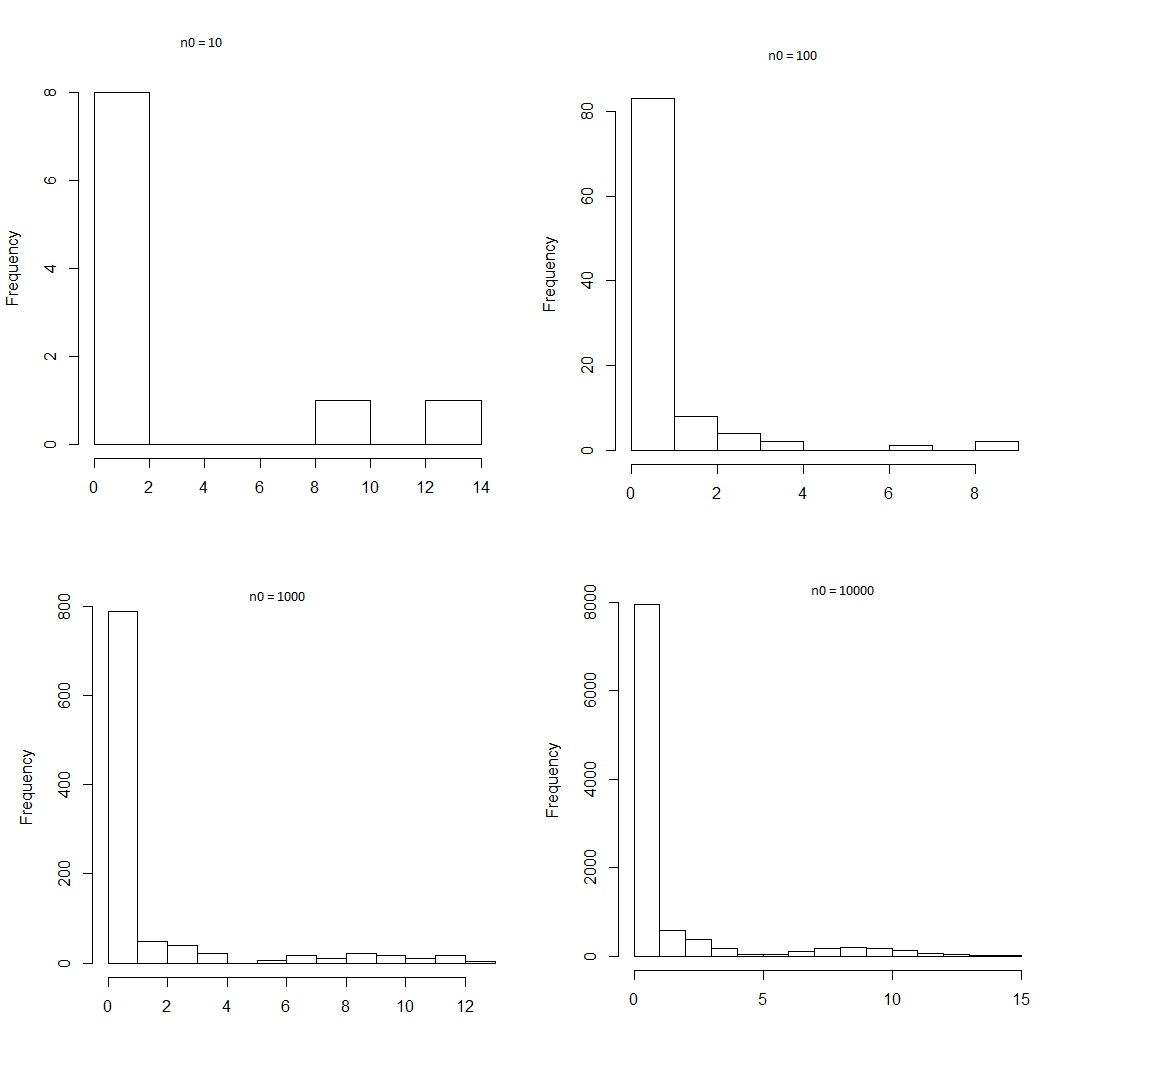
\includegraphics[width=1.2\textwidth]{n0.jpg}
\caption{\label{fig:garf2}Histogramas da distribuição gerada para cada número n0 de iterações para `esquentar a máquina'' com n0=10,100,1000 e 10000, respectivamente'. }
\end{figure}

\begin{figure}
\centering
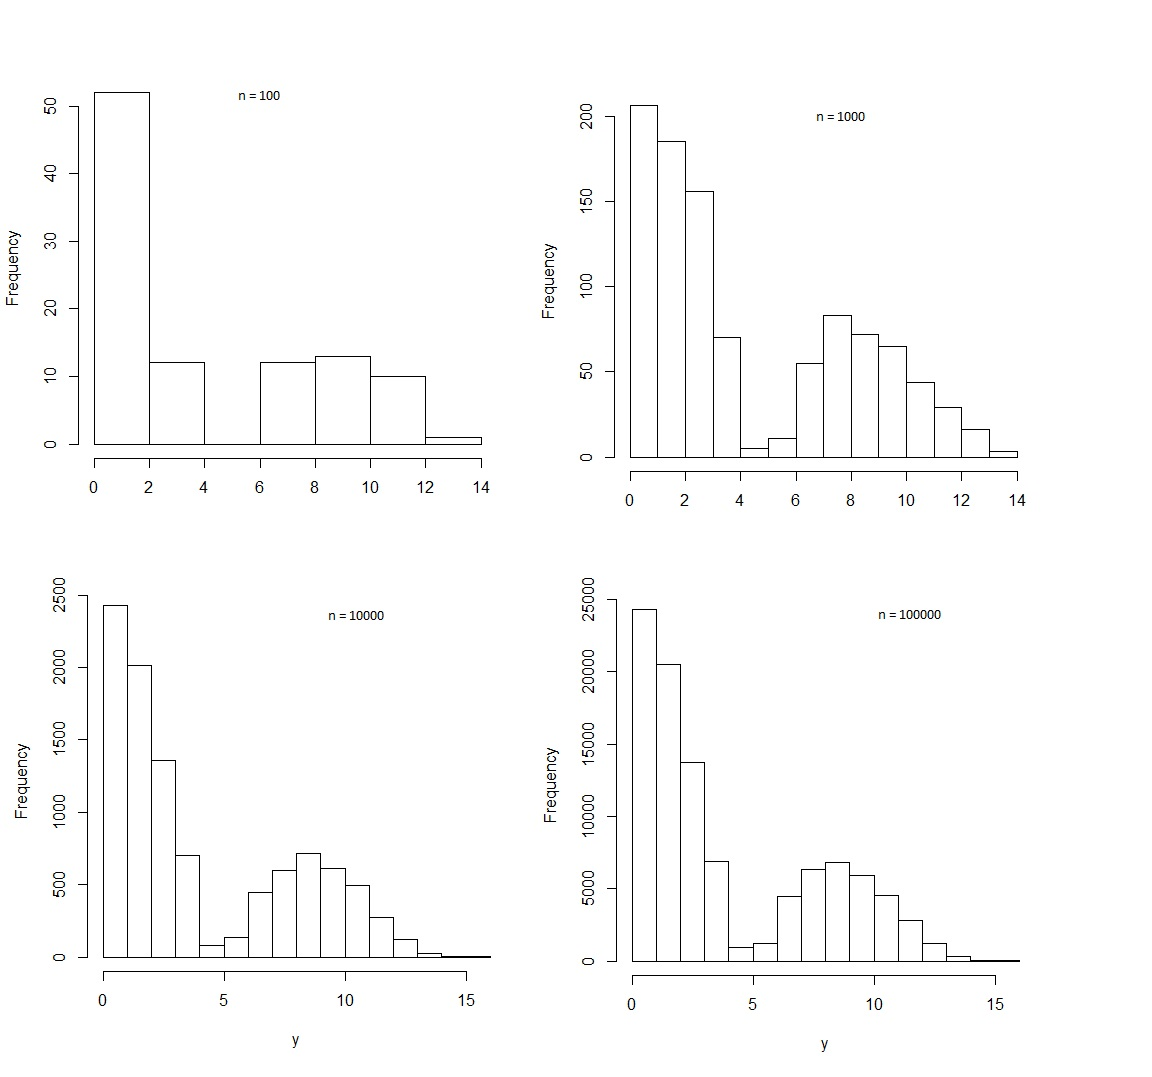
\includegraphics[width=1.2\textwidth]{n.jpg}
\caption{\label{fig:garf2}Histogramas da distribuição gerada para n utilizando-se do núcleo normal para diversos tamanhos de amostra n=100,1000,10000 e 100000, respectivamente. }
\end{figure}

\begin{figure}
\centering
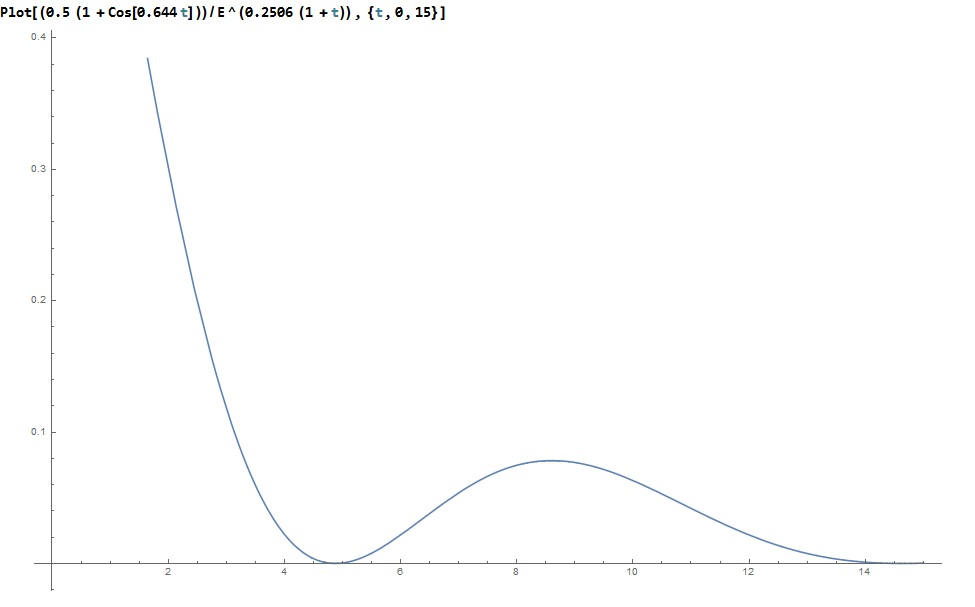
\includegraphics[width=1.2\textwidth]{g.jpg}
\caption{\label{fig:garf2}Gráfico de g em [0,15]. }
\end{figure}

\section{Conclusões}
A figura 3 mostra um esboço do gráfico da função $g$. Através destes gráficos é possível verificar, ao menos qualitativamente, que o método gera números com distribuição similar à da função $g$.
 
 As integrais foram estimadas usando a relação:
\[ \int_0^\infty f(t)g(t)dt=\dfrac{1}{N} \sum{h(x_i)} \]
com  $x_g$ sendo a variável aleatória com distribuição $g$ gerada pelo algoritmo de Metropolis-Hastings.
Executando o algoritmo para 10000 pontos, obtivemos
\[ \int_0^\infty f(t)g(t)dt \approx 1.722\]

\end{document}
